\section{Laser 635\,nm}
\begin{table}
\begin{center}
\caption{ Wyznaczone wartośc prądu progowego $I_{\mathrm{th}}$ w różnych temperaturach $T$ dla lasera krawędziowego 635\,nm. }
\begin{tabular}{ | C{1.5cm}|  C{1.5cm} | C{1.5cm} | C{1.5cm}| C{1.5cm} | C{1.5cm}| C{1.5cm}| C{2.0cm}| C{2.0cm}|}
\hline
$T$ [K] 	&   278 & 283  	& 288 & 293 & 298 & 303 & 308 \\ \hline
$I_{\mathrm{th}}$ [mA]  &	19.1 $\pm$ 0.2  & 20.7 $\pm$ 0.2 & 22.6 $\pm$ 0.2 &
25.0 $\pm$ 0.2  & 27.9 $\pm$ 0.3 & 31.4 $\pm$ 0.5 & 36 $\pm$ 2	\\ \hline
\end{tabular}
\end{center}
\end{table}
\begin{figure}
\center
  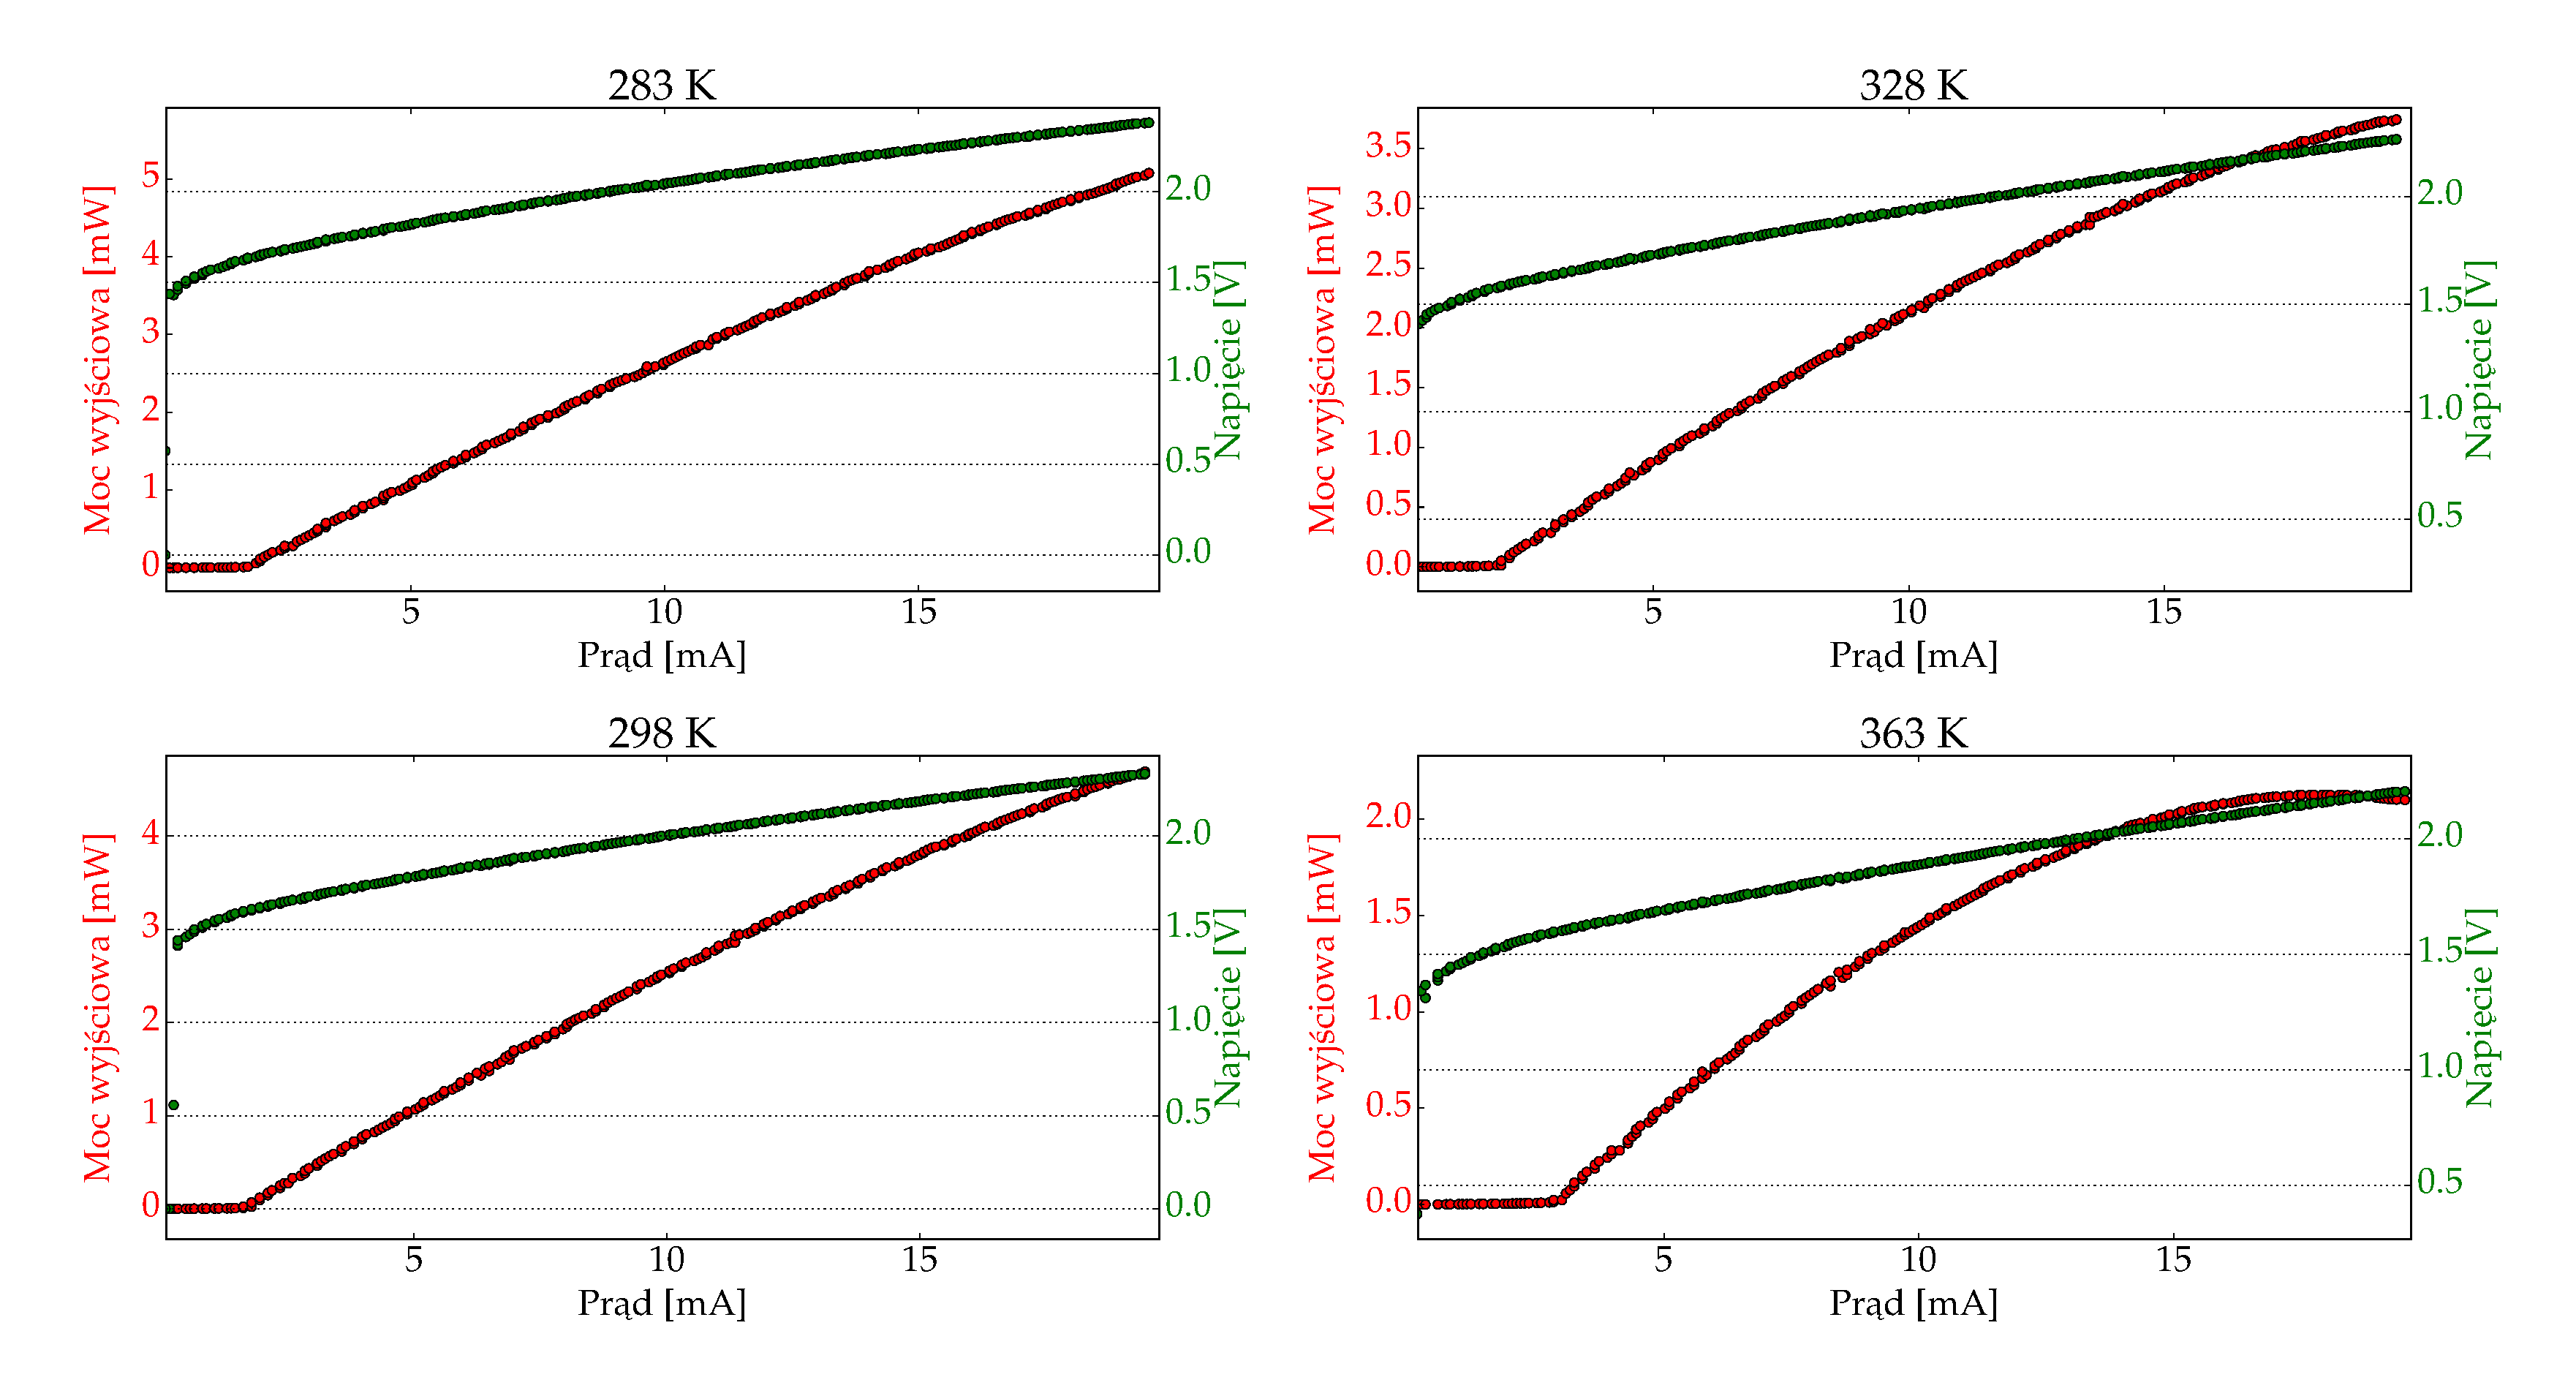
\includegraphics[scale=0.30]{plot635/plot_ivl_4.eps}
  \label{rys1}
  \caption{Wykres napięcia i mocy od prądu dla lasera krawędziowego 635\,nm.}
\end{figure}
\begin{figure}
\center
  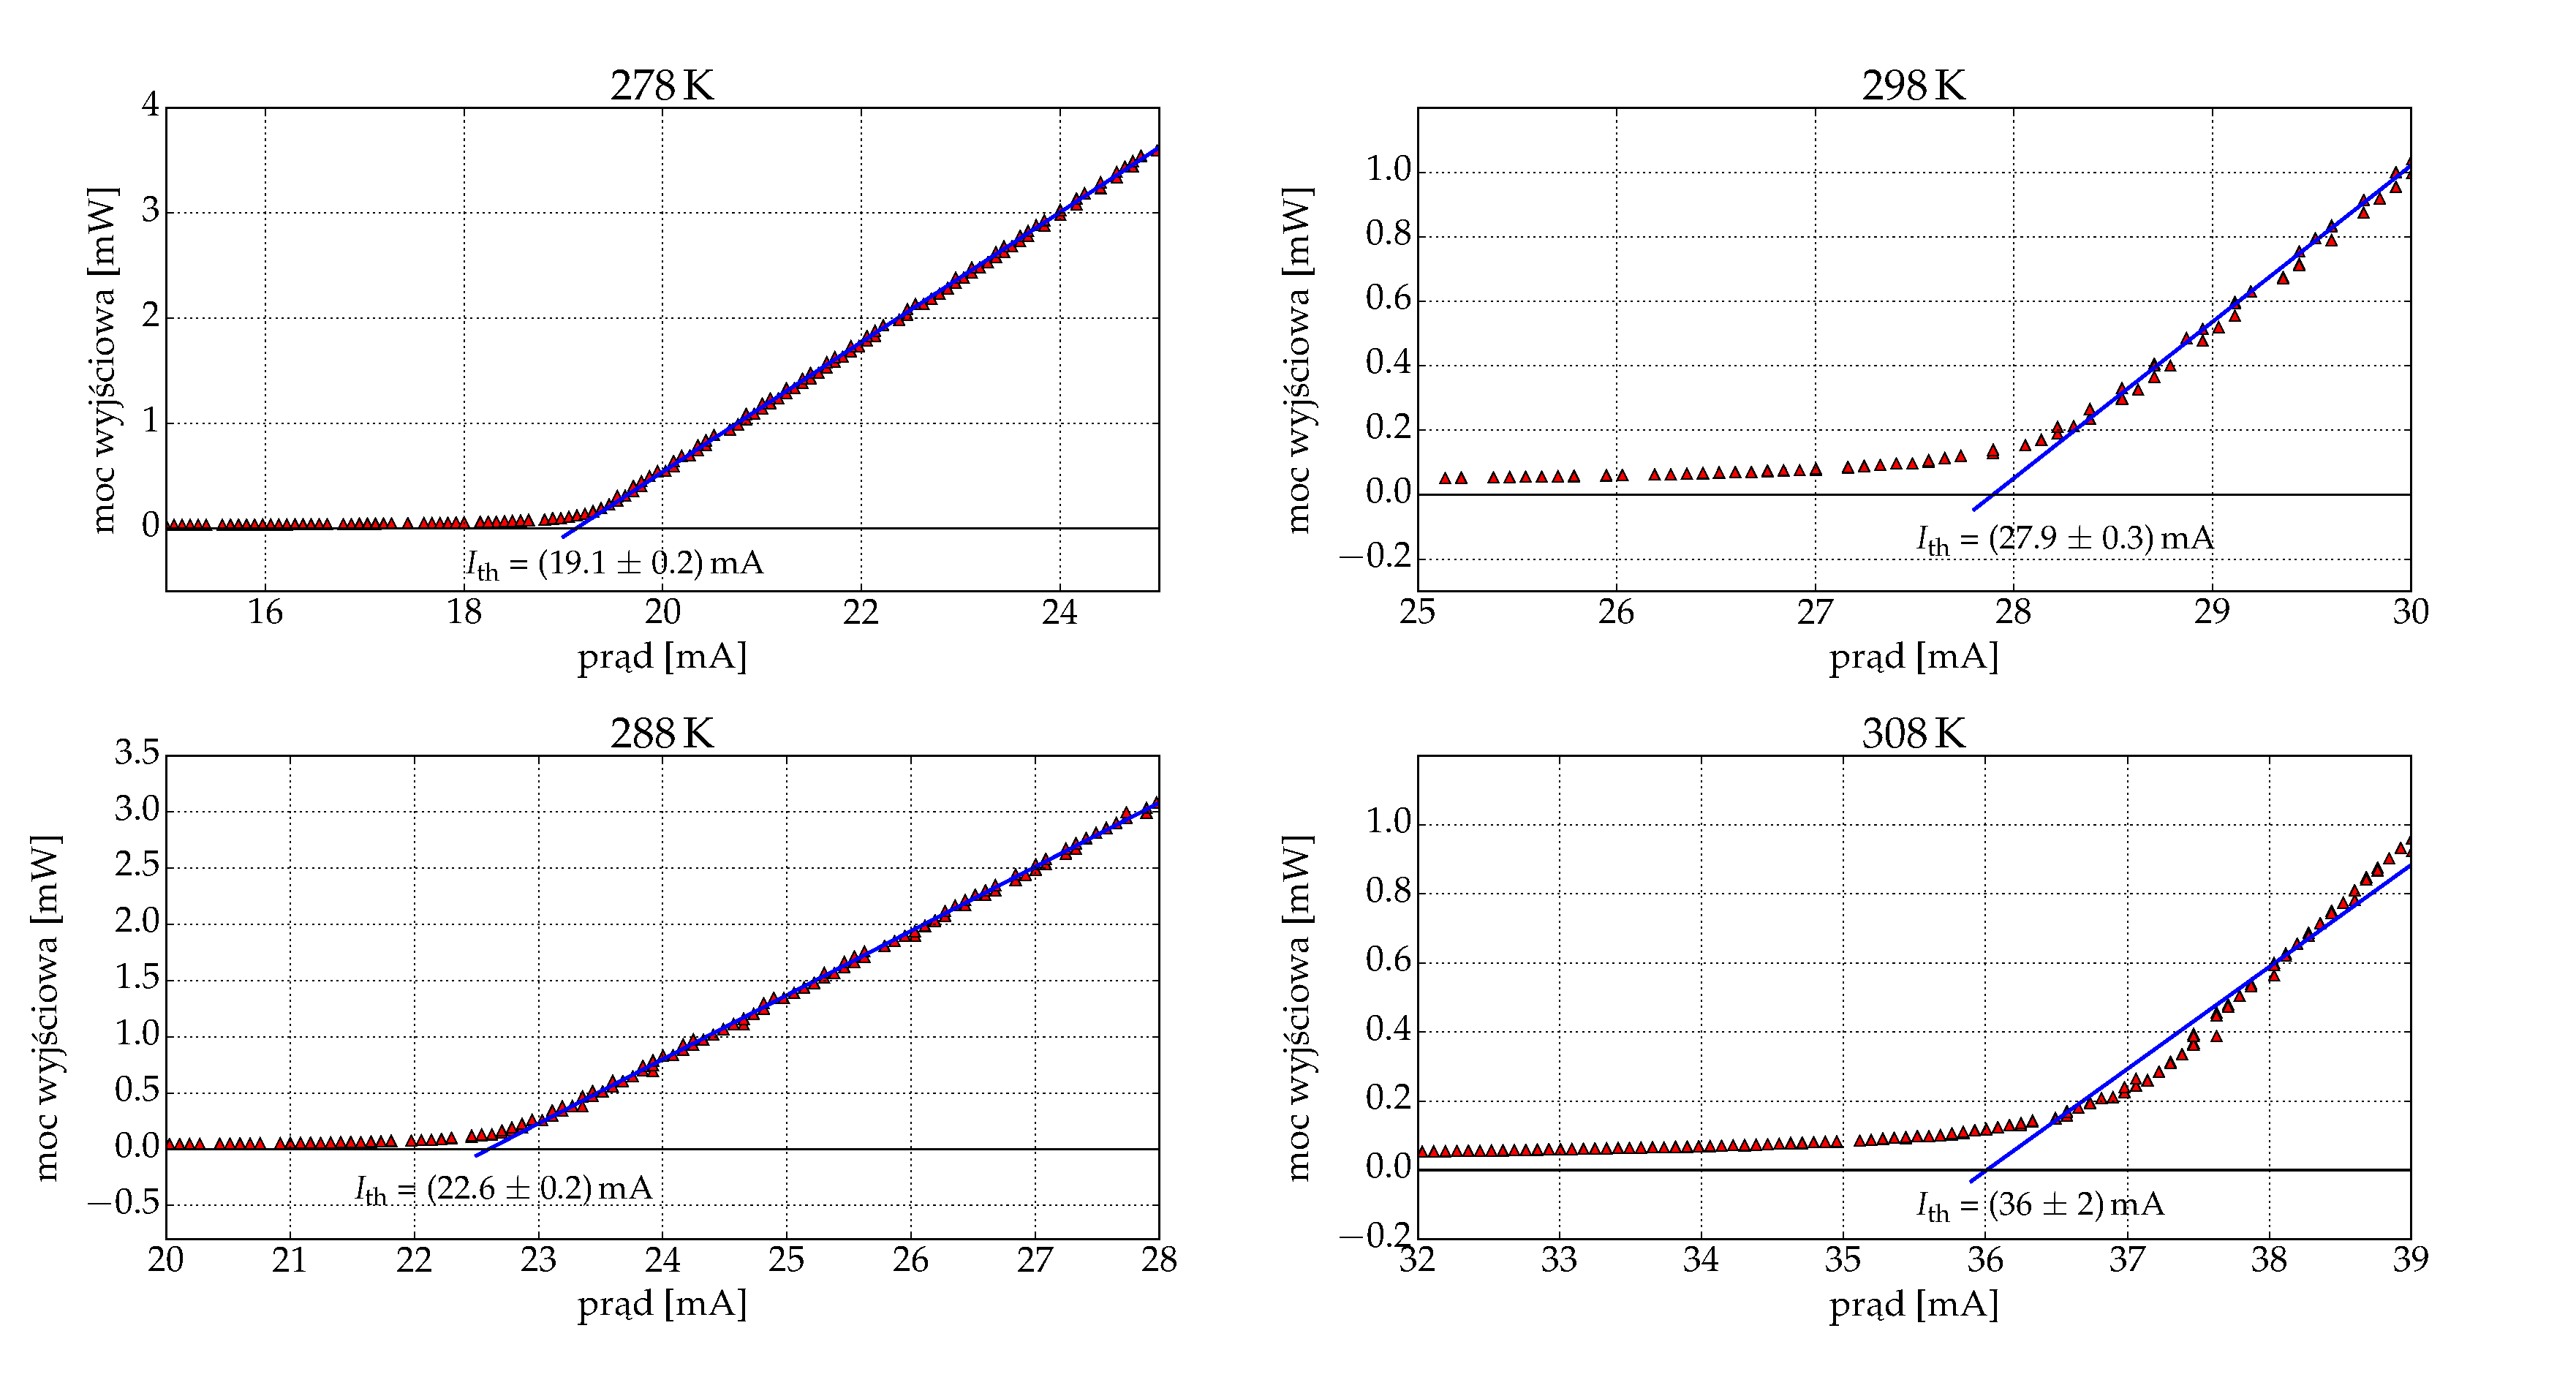
\includegraphics[scale=0.30]{plot635/plot_i_th_4.eps}
  \label{rys2}
  \caption{Wykres prądu progowego dla lasera krawędziowego 635\,nm.}
\end{figure}
\begin{figure}
\center
  % This file was created by matplotlib2tikz v0.6.0.
\begin{tikzpicture}

\begin{axis}[
xlabel={Temperatura [K]},
ylabel={Prąd progowy [mA]},
xmin=275, xmax=310,
ymin=15, ymax=40,
axis on top,
width=15cm,
height=8cm,
xmajorgrids,
ymajorgrids
]
\path [draw=red] (axis cs:278,18.9)
--(axis cs:278,19.3);

\path [draw=red] (axis cs:283,20.5)
--(axis cs:283,20.9);

\path [draw=red] (axis cs:288,22.4)
--(axis cs:288,22.8);

\path [draw=red] (axis cs:293,24.8)
--(axis cs:293,25.2);

\path [draw=red] (axis cs:298,27.6)
--(axis cs:298,28.2);

\path [draw=red] (axis cs:303,30.9)
--(axis cs:303,31.9);

\path [draw=red] (axis cs:308,34)
--(axis cs:308,38);

\addplot [red, mark=-, mark size=3, mark options={solid}, only marks]
table {%
278 18.9
283 20.5
288 22.4
293 24.8
298 27.6
303 30.9
308 34
};
\addplot [red, mark=-, mark size=3, mark options={solid}, only marks]
table {%
278 19.3
283 20.9
288 22.8
293 25.2
298 28.2
303 31.9
308 38
};
\addplot [red, mark=*, mark size=1, mark options={solid,draw=black}, only marks]
table {%
278 19.1
283 20.7
288 22.6
293 25
298 27.9
303 31.4
308 36
};
\end{axis}

\end{tikzpicture}
  \label{rys2}
  \caption{Wykres prądu progowego od temperatury dla lasera krawędziowego 635\,nm.}
\end{figure}
\begin{figure}
\center
  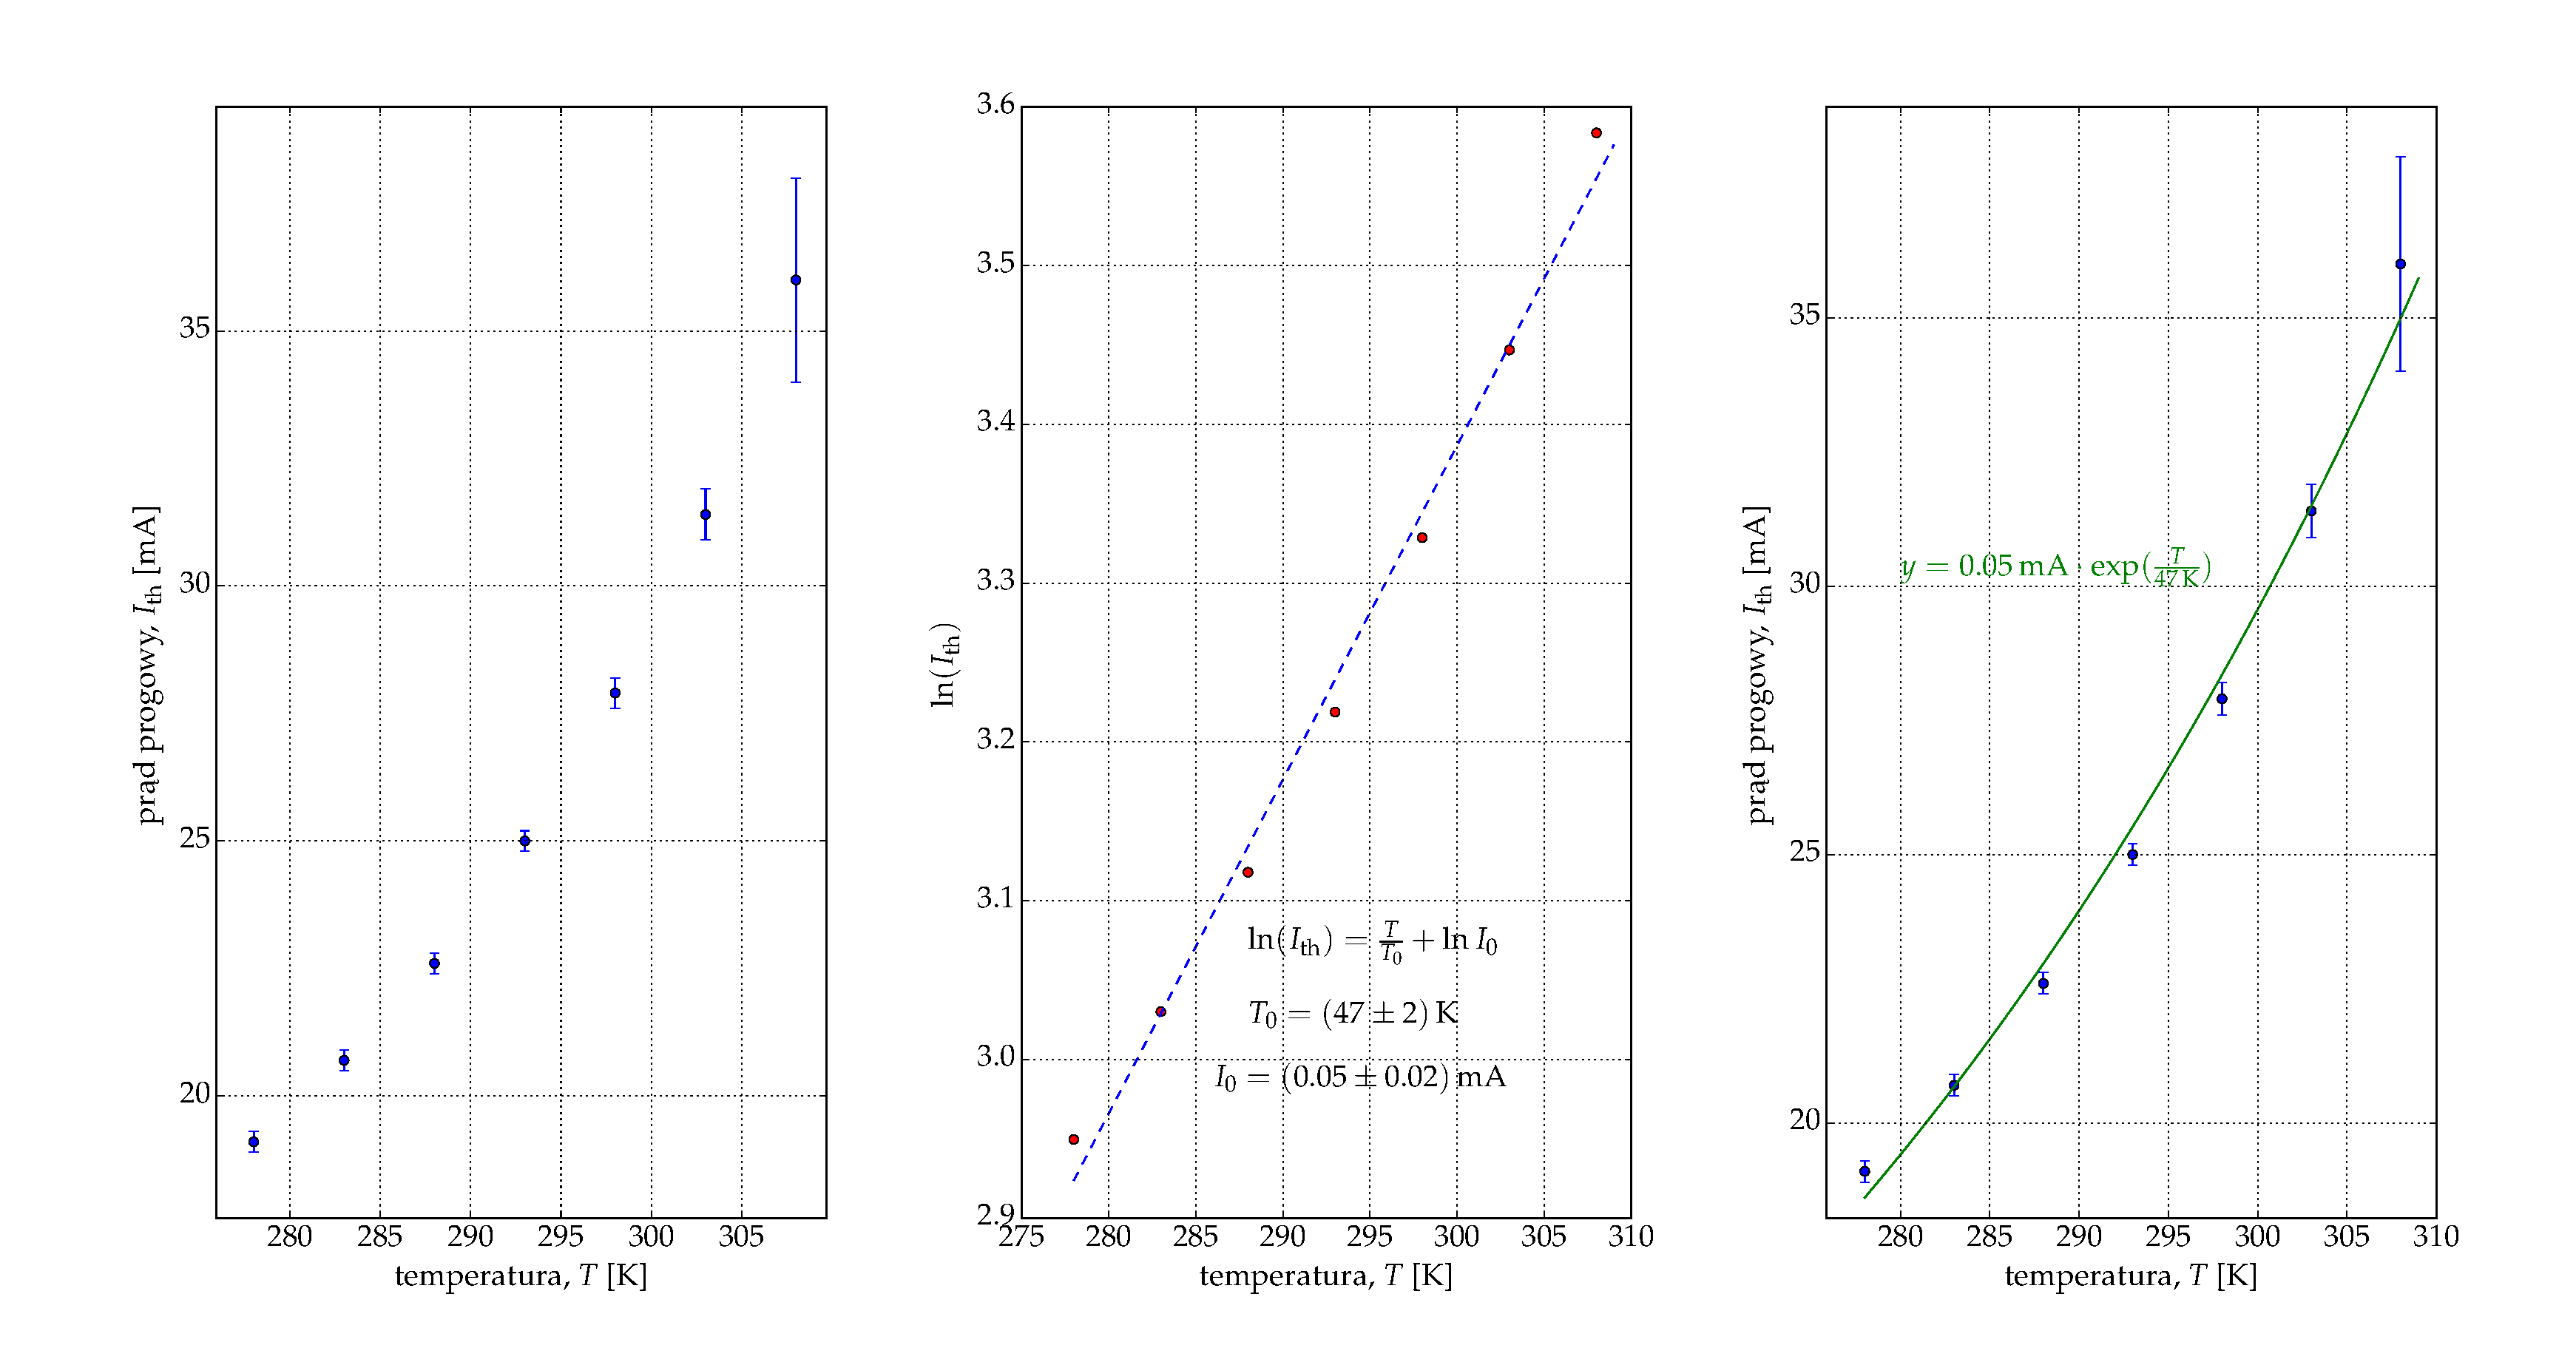
\includegraphics[scale=0.30]{plot635/plot_fit.eps}
  \label{rys2}
  \caption{Wykres prądu progowego z dopasowanymi wartościami $I_{0}$ i $T_{0}$ dla lasera krawędziowego 635\,nm.}
\end{figure}
\begin{figure}
\center
  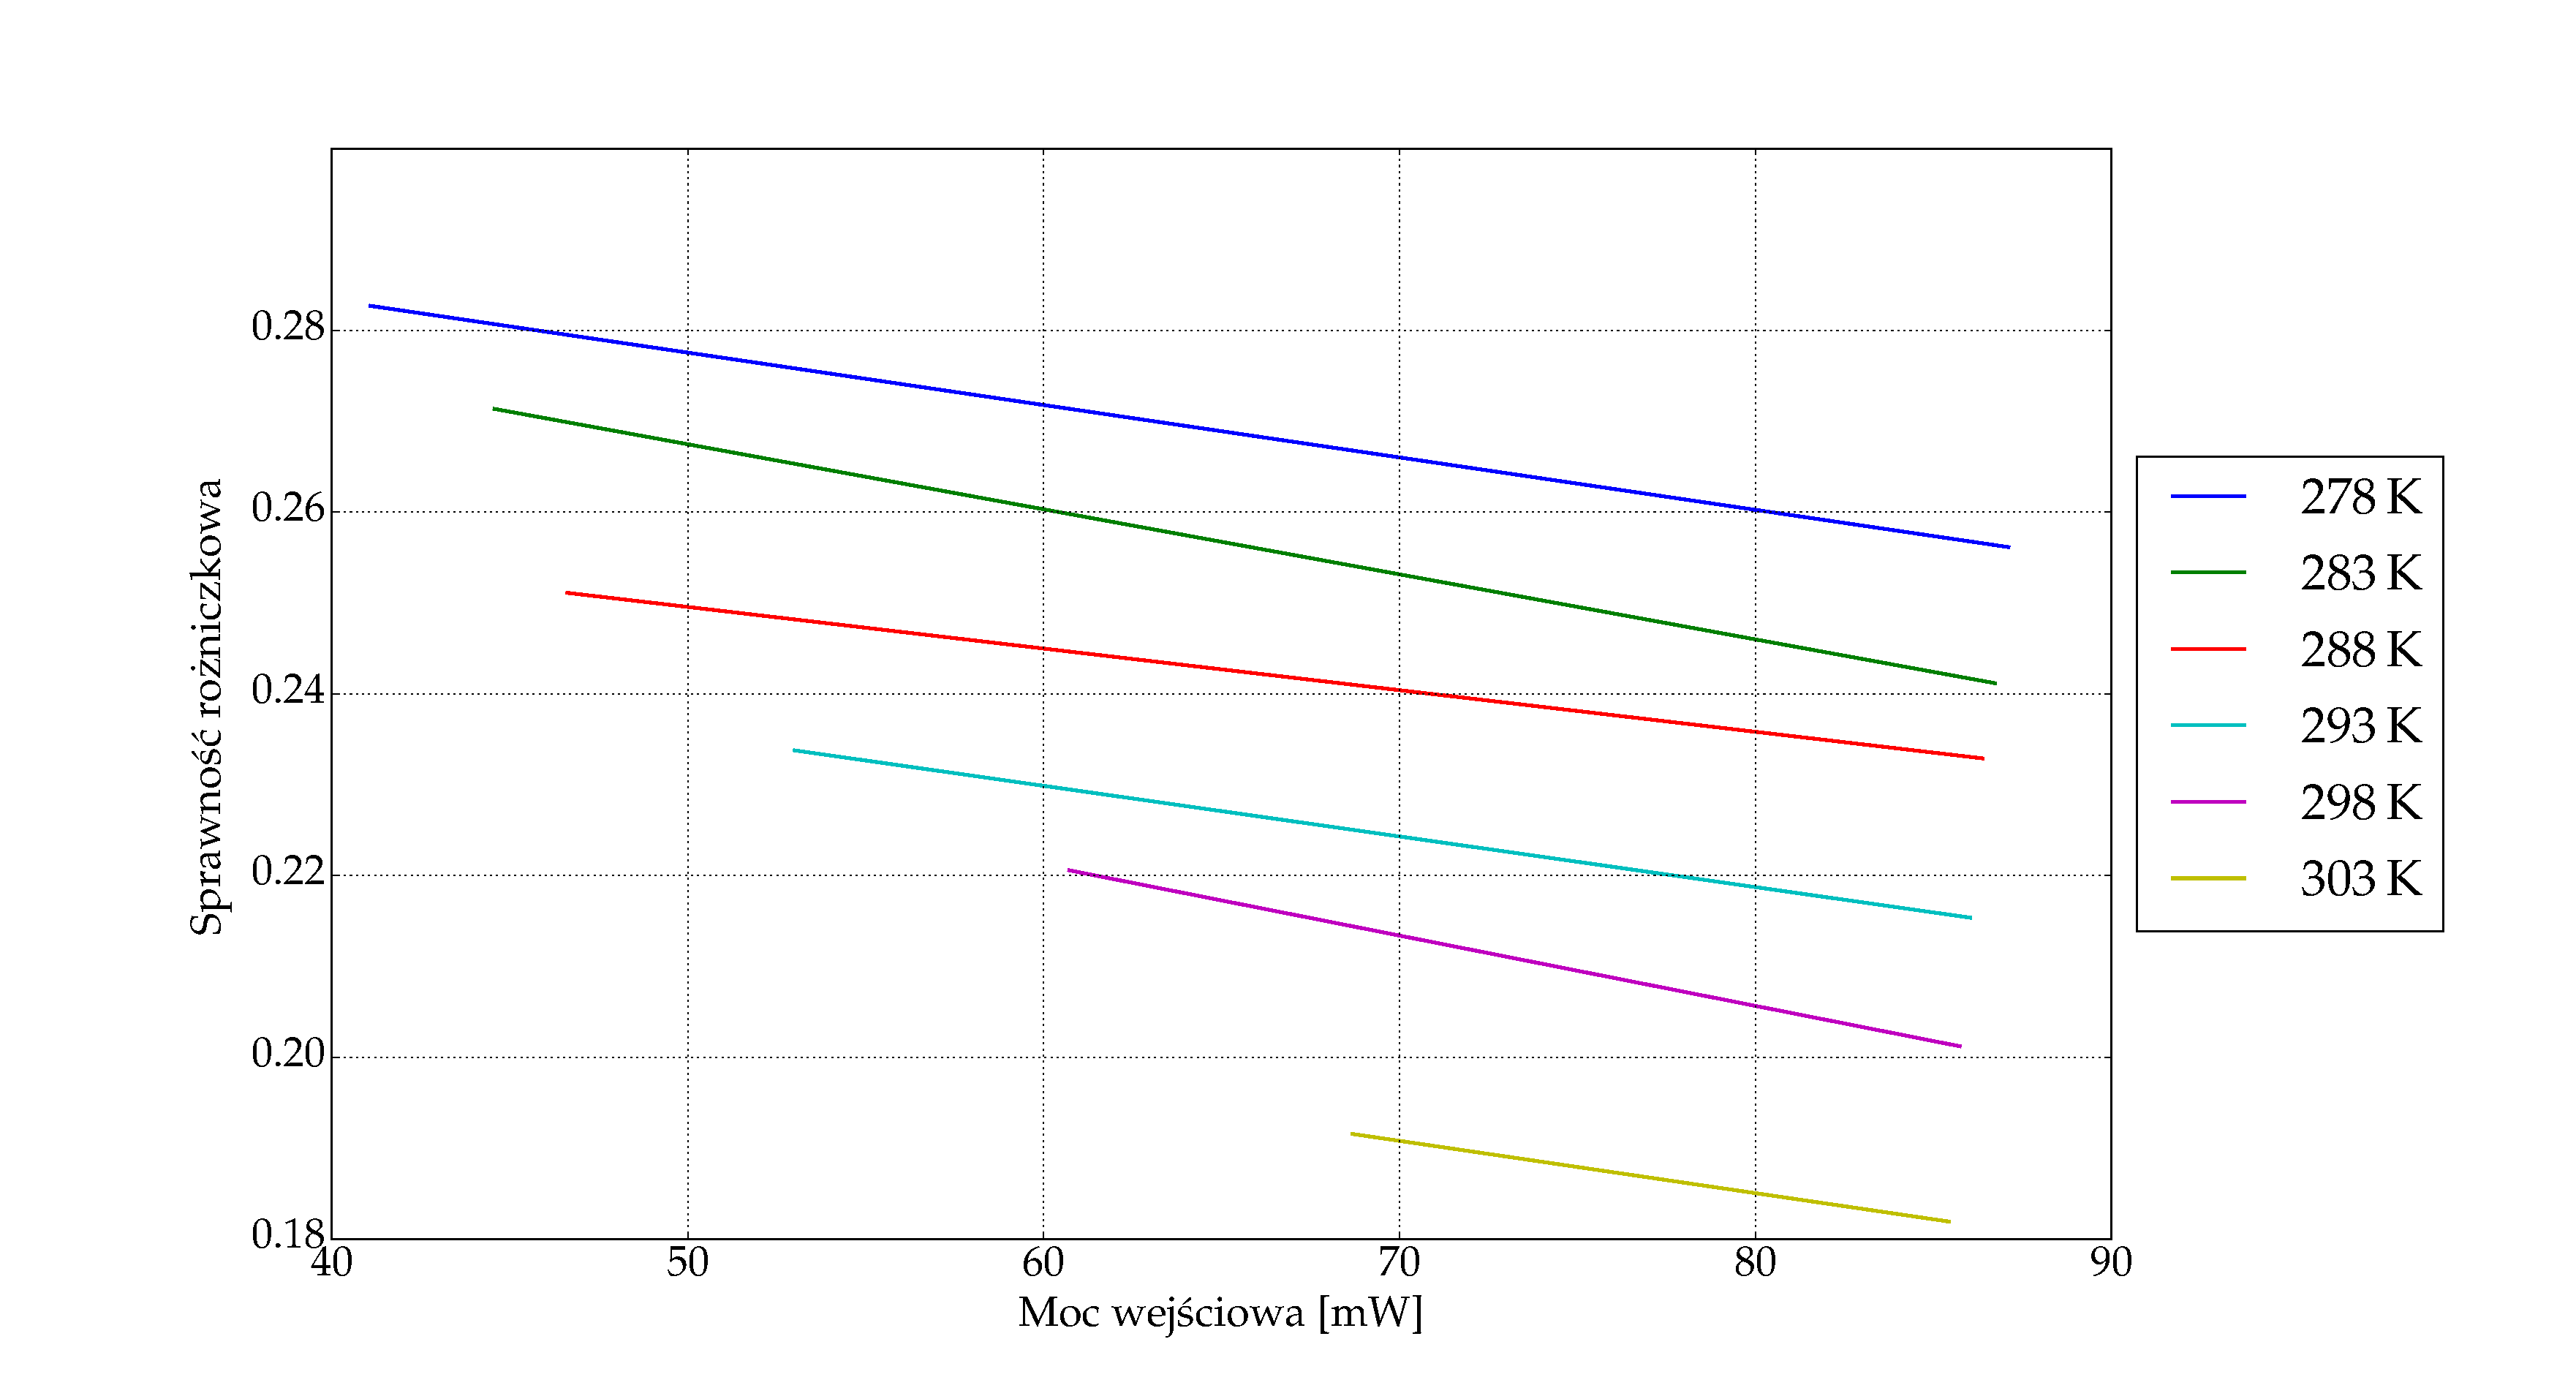
\includegraphics[scale=0.30]{plot635/plot_eff_via_power.eps}
  \label{rys3}
  \caption{Wykres sprawności w funkcji mocy wejściowej dla lasera krawędziowego 635\,nm.}
\end{figure}
\begin{figure}
\center
  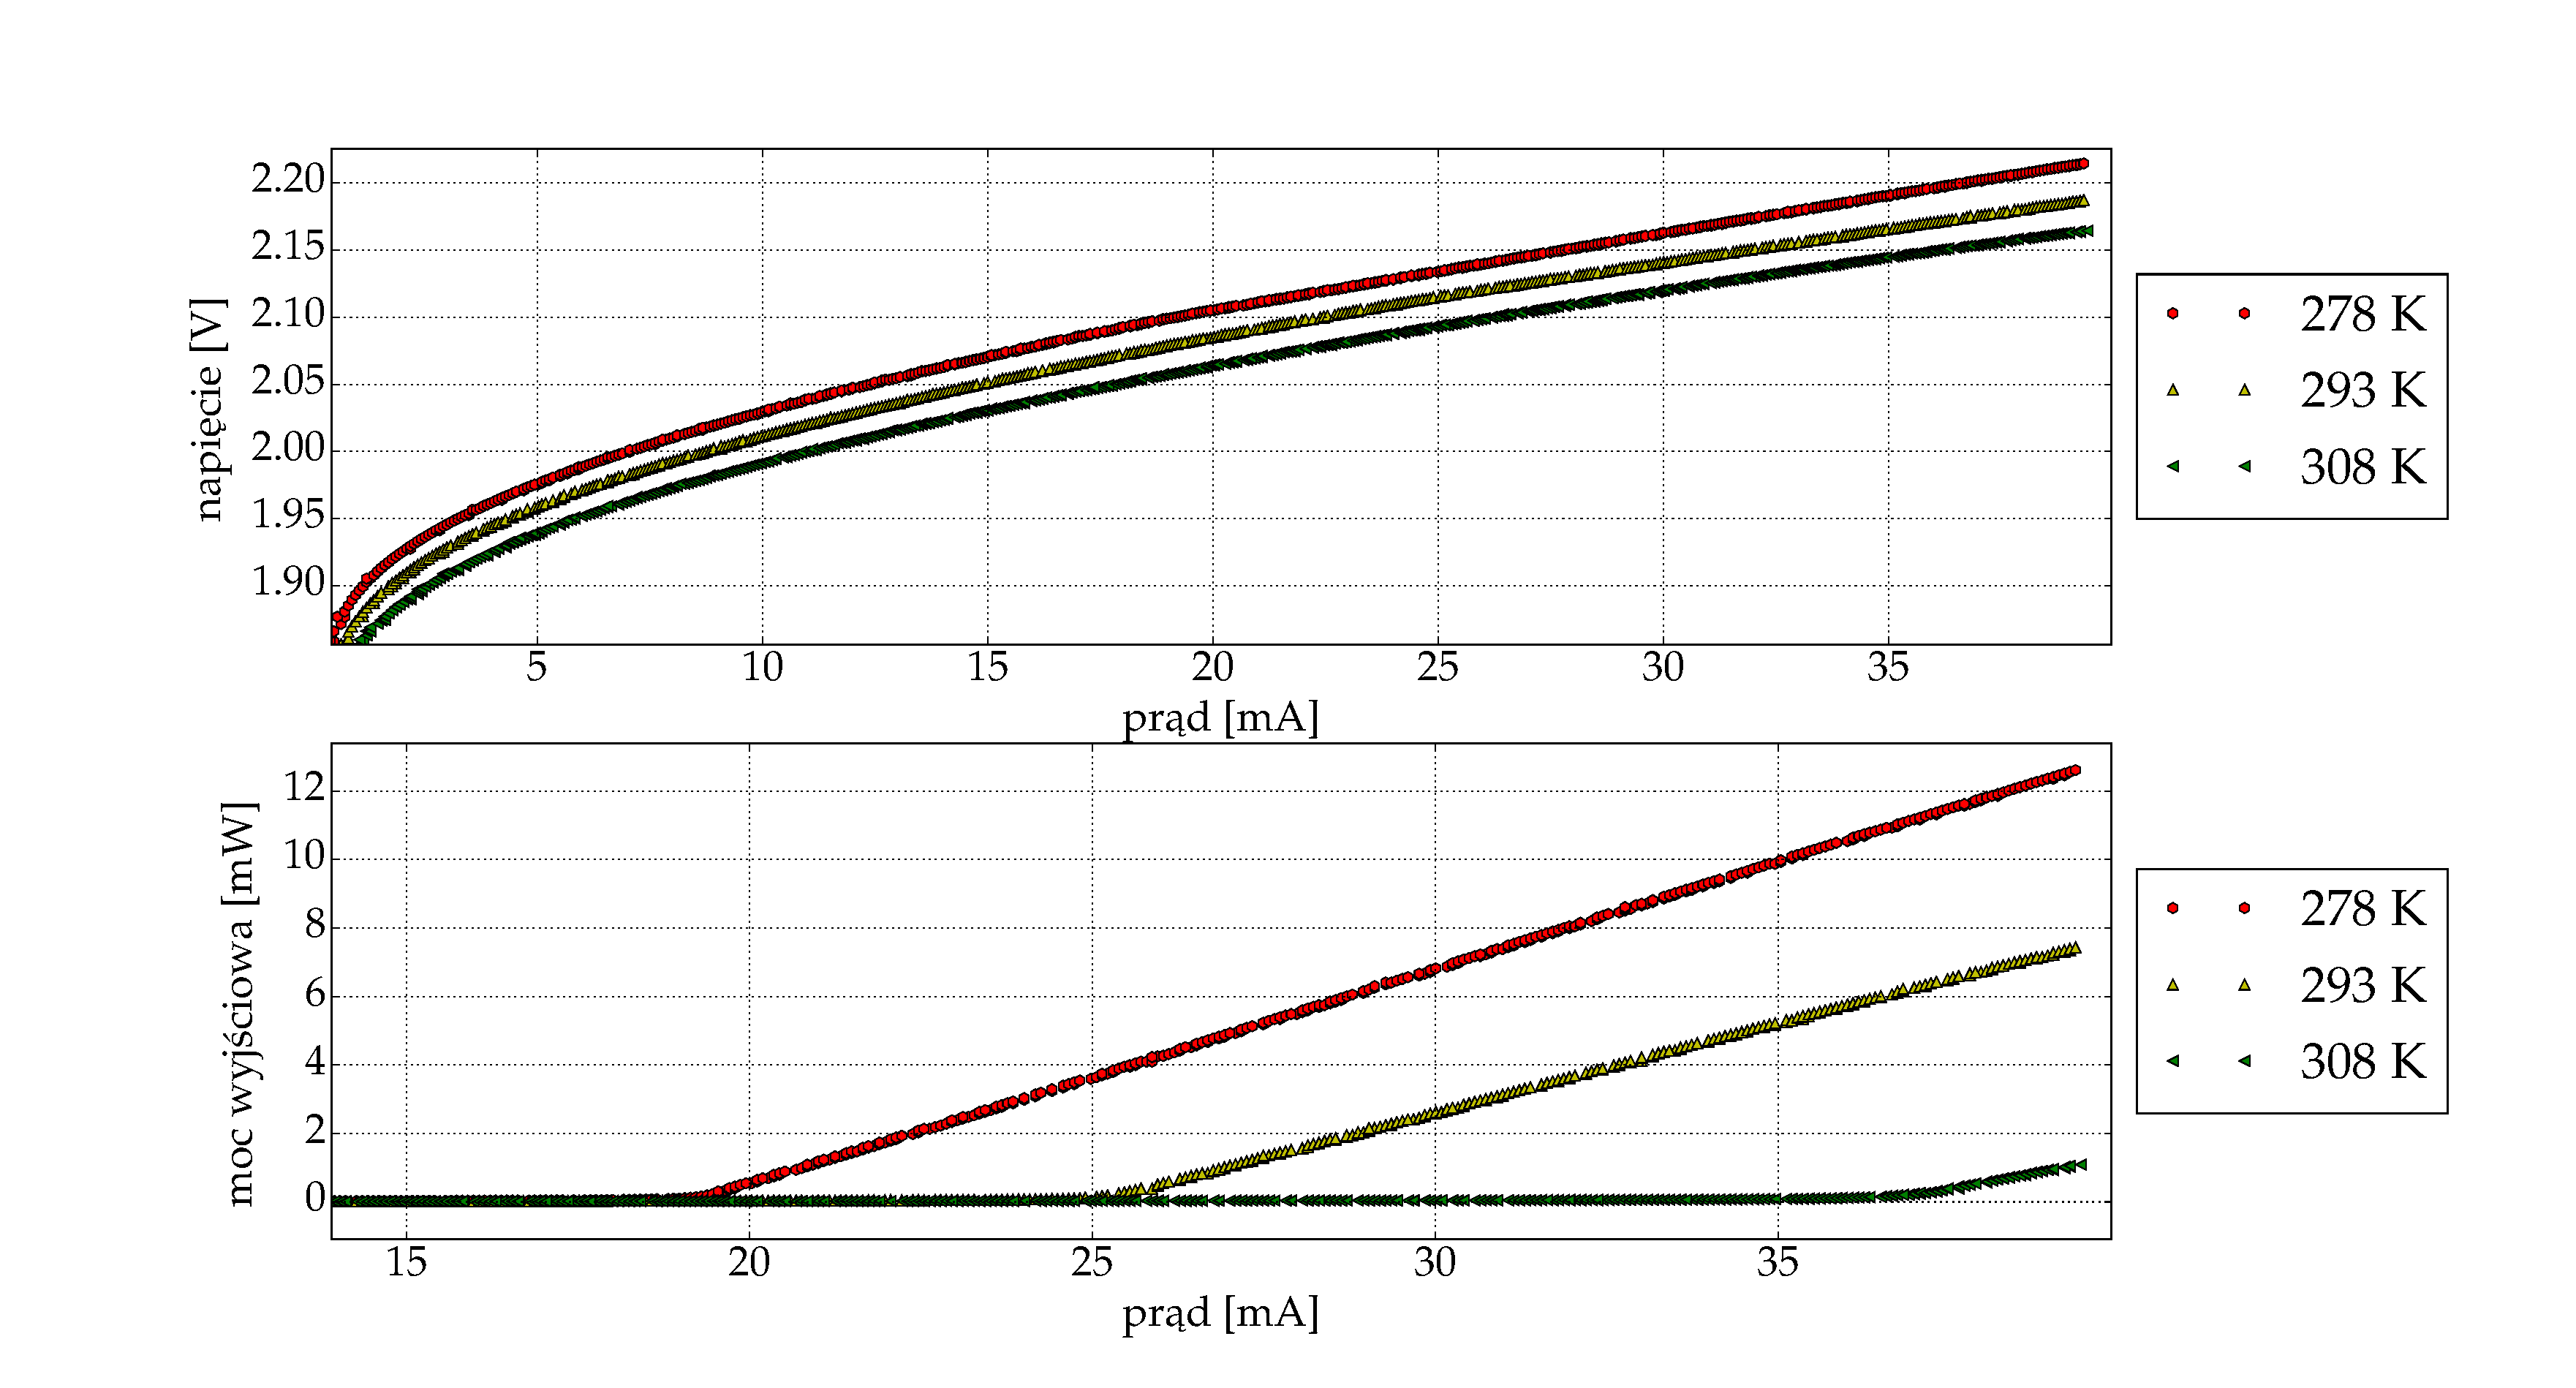
\includegraphics[scale=0.30]{plot635/plot_voltage_power.eps}
  \label{rys3}
  \caption{Wykres napięcia na laserze oraz mocy w funkcji prądu dla lasera krawędziowego 635\,nm.}
\end{figure}
